\documentclass{article}
\usepackage{iclr2026_conference,times}
\usepackage{graphicx,booktabs,hyperref}
\hypersetup{hidelinks}
\iclrfinalcopy
\title{Budgeted Bitemporal Source Memory in JiuwenSwarm: A Controlled Study}
\author{Anonymous Competition Research System}
\begin{document}
\maketitle
\fancyhead[L]{Controlled engineering study -- external evaluation pending}
\begin{abstract}
Selecting memory for an agent requires deciding which source records remain relevant under temporal updates and a restricted context window. We implement an opt-in JiuwenSwarm Rail that filters structured facts by effective and observation times, preserves maximal-time conflict groups atomically and packs original evidence under a selected-context budget. Bitemporal modeling is established prior art \citep{temporal}; the contribution is a reusable framework extension and a traceable controlled evaluation. A fixed ReActAgent is compared across recency, lexical, BM25, summary, full-history and temporal/conflict ablation conditions. All bounded methods share a source-context limit, while total provider usage includes instructions, answers and summary calls. Measured outcomes are reported separately from evidence availability, including null ablation outcomes. The study uses synthetic records with explicit metadata, no tools and no free-text ingestion. It supplies reproducible engineering evidence rather than a claim of superiority over general long-term memory systems.
\end{abstract}
\begin{figure}[ht]\centering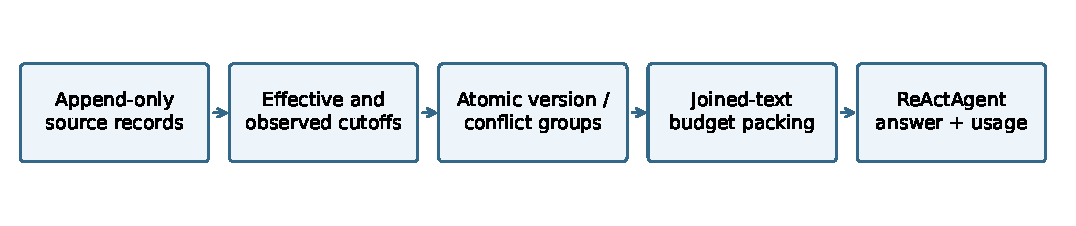
\includegraphics[width=\linewidth]{architecture.pdf}
\caption{Source-evidence selection and invocation accounting. The memory layer returns original records, not gold answers.}\end{figure}
\section{Introduction}
An agent reading an evolving record stream must distinguish when a fact applies from when the system learned it. Late observations of old facts, unresolved contradictions and deletions can make naive context selection misleading even when lexical matching succeeds. A restricted context window adds a second problem: evidence about different requested attributes competes for space. We study that engineering problem with explicit structured records and a fixed answering model.

Our contribution is an opt-in JiuwenSwarm source-memory Rail, an append-only record interface and a reproducible evaluation with persisted responses and resource accounting. Bitemporal modeling is established prior art \citep{temporal}; neither its invention nor general superiority over memory systems is claimed. The selectors return original source records, never resolved reference answers. The evaluation includes lexical methods, a full-context reference, and time/conflict ablations. All bounded methods share a selected-source-context limit; total API cost is measured separately. The structured input assumption deliberately excludes free-text extraction and is a major limit on deployment claims. LongMemEval illustrates the broader interactive setting that still requires external validation \citep{longmemeval}.
\section{Related Work}
Bitemporal modeling and per-attribute version filtering are established ideas. Valid time and transaction time were articulated in temporal database work \citep{temporal}, and our study does not invent bitemporal modeling; it adopts these concepts as an engineering substrate. Memory-augmented agent systems such as MemGPT study virtual context management with hierarchical memory \citep{memgpt}, while Mem0 extracts, consolidates, and retrieves long-term memories and studies a graph extension \citep{memzero}, and A-MEM dynamically links structured notes and evolves memory representations \citep{amem}. These systems are related work only; we do not reproduce their implementations, and we make no comparison to their reported results. Long-term interactive memory benchmarks such as LongMemEval motivate external validation \citep{longmemeval}, but our protocol uses synthetic structured records rather than free-text dialogue, so it should not be read as a dialogue-memory benchmark. Workflow designs for agentic research assistants, including staged literature review, experimentation, and report writing in Agent Laboratory \citep{agentlab} and orchestration of scientific investigation in AI-Researcher \citep{airesearcher}, inform how we separate evidence handling from answer generation; we borrow design ideas, not source code. Our contribution is narrower than any of these systems: a reusable opt-in source-evidence Rail within JiuwenSwarm, together with a controlled and logged evaluation that makes the selected evidence inspectable. We deliberately avoid novelty and state-of-the-art claims, and we treat the lexical ranking function as a stronger lexical baseline rather than as a semantic embedding retriever.
\section{Methods}
Each source record contains a unique local identifier, an entity, a single attribute, a scalar value, an effective-time point named valid\_at, an observation-time point named observed\_at, and a set or delete operation. There are no validity intervals in this implementation. The append-only store preserves original records and supports JSONL round trips. Query metadata supplies the entity, requested attributes and both time cutoffs equally to every method. Visible records satisfy both cutoffs. For each requested attribute, the versioned selector retains the records at the maximal visible effective time. Different values or a set/delete disagreement at that time form an unresolved conflict. Such a group is atomic: it is retained together or omitted together. A tombstone is source evidence for deletion, not an inferred replacement value.

Versioned selection packs smaller complete attribute groups first, breaking equal-cost ties in query order and restoring source order in the final context. Joined JSONL text is recounted after each addition. This greedy rule is not claimed optimal for arbitrary nonadditive tokenizers. The no-time ablation keeps the observation cutoff but orders and selects by observation time rather than effective time. The no-conflict ablation keeps both cutoffs and maximal effective time, then breaks ties by latest observation; it does not discard every conflicting record.

Full history passes the unbounded source stream. Recent selection uses a contiguous suffix. Lexical overlap and BM25 rank serialized source records using the entity, requested attributes and question text. They receive the same metadata as the structured selectors but do not use temporal filtering in their ranking. Lexical-summary compresses the already retrieved lexical records, not discarded records, and truncates the summary to the same selected-context limit. Summary calls add to total API consumption; they do not make total call budgets equal.

A fresh openJiuwen ReActAgent receives the selected context and the common query semantics. The Rail injects context before invocation and records the model response before later agent postprocessing. Requests are reserved durably before transport and reconciled to provider usage. Unknown spend blocks further calls. Answer accuracy requires the exact requested JSON keys and type-correct values. Micro-field accuracy pools correct fields. Stale-field counts compare nonnull returned values to superseded visible source values. Evidence recall measures reference record identifiers available in the selected source context, not model-provided citations. For summary methods it describes the retrieved source records and does not certify compression faithfulness. Metadata extraction requires no model call here because it is an input assumption.
\subsection{Frozen Protocol}
The fixed protocol uses six development tasks and twenty-four held-out tasks, with disjoint seed namespaces and six task families. All methods receive identical structured records, query metadata and answering instructions. The primary selected-context budget is 256 cl100k\_base proxy tokens. A 512-token sensitivity comparison uses twelve fixed held-out tasks; full history is an unbounded reference evaluated only in the primary grid. The frozen grid has 324 task-policy-budget outcomes. Each answering session is isolated, uses temperature zero, disables thinking and tools, and allows 160 output tokens. Lexical summary allows an additional 256-token model output before truncation to the selected-context budget. API-reported usage, including summary overhead, is the cost measure; proxy context length is not provider billing. Retrieval ties and source ordering are deterministic. BM25 here is strictly lexical; no semantic embedding retriever is evaluated.
\section{Measured Results}
\begin{table}[ht]\centering\small
\begin{tabular}{lrrrr}\toprule
Policy & Correct & Exact (\%) & Field (\%) & Tokens \\ \midrule
bm25 & 6/24 & 25.0 & 56.6 & 12180 \\
full & 18/24 & 75.0 & 86.8 & 40860 \\
lexical & 18/24 & 75.0 & 92.1 & 12240 \\
lexical\_summary & 13/24 & 54.2 & 81.6 & 26402 \\
no\_conflict & 20/24 & 83.3 & 94.7 & 9440 \\
no\_time & 8/24 & 33.3 & 47.4 & 9386 \\
recent & 0/24 & 0.0 & 15.8 & 12195 \\
versioned & 20/24 & 83.3 & 94.7 & 9592 \\
\bottomrule\end{tabular}
\caption{Held-out primary comparison. Full history is unbounded; other methods share the selected-context budget. Tokens include summary calls.}\end{table}
\begin{figure}[ht]\centering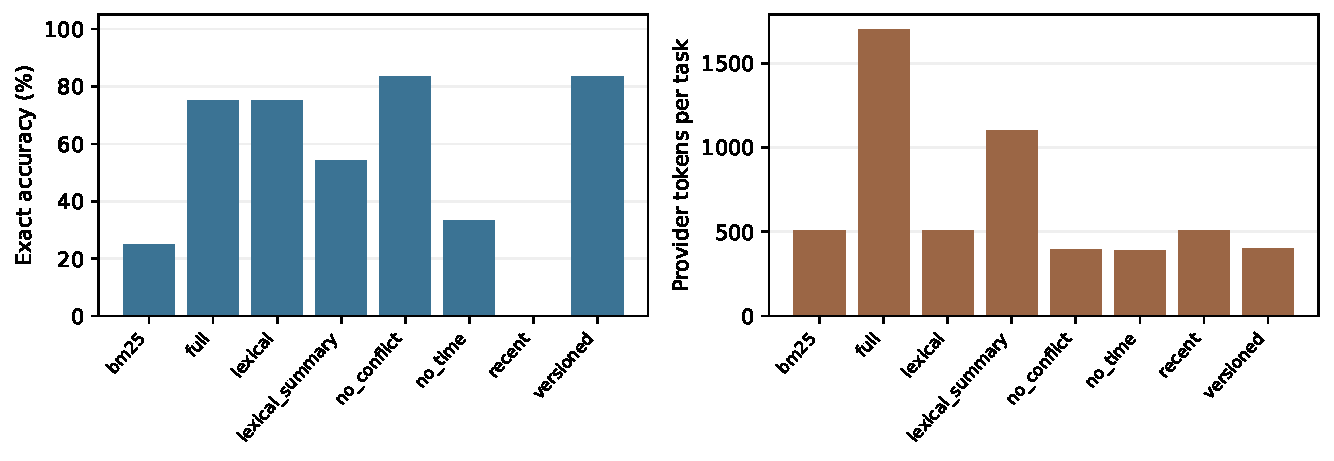
\includegraphics[width=\linewidth]{results.pdf}
\caption{Primary held-out exact accuracy and provider tokens per task. Point estimates describe this controlled sample.}\end{figure}
\begin{table}[ht]\centering\small
\begin{tabular}{lrr}\toprule
Policy & Correct & Exact (\%) \\ \midrule
bm25 & 7/12 & 58.3 \\
lexical & 9/12 & 75.0 \\
lexical\_summary & 7/12 & 58.3 \\
no\_conflict & 10/12 & 83.3 \\
no\_time & 4/12 & 33.3 \\
recent & 0/12 & 0.0 \\
versioned & 10/12 & 83.3 \\
\bottomrule\end{tabular}
\caption{Larger-budget sensitivity on the same fixed subset across bounded methods; this sample differs from the primary table.}\end{table}
Versioned and no-conflict selection tie at 20/24 exact answers. Thus this run provides no observed accuracy gain from atomic conflict preservation. The versioned method retains all reference source evidence at the primary budget but the model still makes errors; evidence sufficiency does not guarantee correct conflict interpretation.
\begin{table}[ht]\centering\small
\begin{tabular}{lrrr}\toprule
Comparator & Tasks & Difference (pp) & Interval (pp) \\ \midrule
full & 24 & 8.3 & [-3.0, 19.6] \\
lexical & 24 & 8.3 & [-3.0, 19.6] \\
no\_conflict & 24 & 0.0 & [0.0, 0.0] \\
\bottomrule\end{tabular}
\caption{Exploratory paired normal intervals on task differences. Small related synthetic cases and unadjusted comparisons preclude significance or generalization claims.}\end{table}
\section{Discussion}
The measured tables describe a single fixed set of model responses, not a robust ranking across models or independent repeated samplings. In particular, the full-context reference is unbounded and must not be described as having the same total cost as a bounded method. Equal selected source-context limits isolate packing behavior; instruction tokens, answer tokens and additional summary calls remain visible in provider accounting. Differences in these costs are outcomes, not violations of the selected-context definition.

The conflict ablation is important because preserving contradictory source records and correctly interpreting them are separate operations. If extra conflict evidence does not improve exact answers, the evidence-preservation mechanism has not established an accuracy benefit. It may still help auditing, but that utility is different from answer correctness. The source audit therefore records both evidence availability and errors instead of treating retrieval recall as a substitute for downstream evaluation.

Several constraints prevent broad conclusions. The record schema and query metadata are given for free; clean temporal annotations would have an extraction cost and failure rate in deployment. The cases are synthetic and closely related within families, and there is only a small held-out sample. Descriptive intervals do not establish significance or external validity. BM25 is lexical; an embedding retriever is absent. No Mem0 or A-MEM implementation is reproduced \citep{memzero,amem}. The answering agent has no tools or iterative action loop. Real-dialogue evaluation, direct citation faithfulness and independent repetitions remain necessary extensions \citep{longmemeval}.
\section{Conclusion}
This work delivers an opt-in bitemporal source-memory extension and a bounded, traceable evaluation workflow for JiuwenSwarm on openJiuwen. It tests engineering mechanisms under explicit structured-input assumptions and reports negative as well as positive observations. Established temporal semantics are credited \citep{temporal}. Source preservation, model answer correctness and API cost are kept separate. The evidence supports a reproducible controlled study; it does not establish a new general memory algorithm or replace external benchmarks and official assessment.
\section{Limitations and Reproducibility Disclosure}
This is an engineering extension and a small synthetic structured-record evaluation, not an evaluation of unstructured conversation ingestion, real tool use or unrestricted long-term assistants. No embedding retrieval or Mem0/A-MEM implementation is reproduced, and bitemporal modeling is established prior art. There is one model response per fixed case, not an independent-model or repeated-sampling robustness study. Related task families and small samples limit uncertainty interpretation. Evidence recall measures source records available in context, not citations produced by the model; summary-source IDs do not prove facts survived compression. Model prose was generated and mechanically checked; measured tables were inserted by code. Codex assisted design, implementation and review. The official Stanford and paper-agent scores for this manuscript are pending. The Rail was loaded from JiuwenSwarm source on the installed openJiuwen ReActAgent; the full desktop Swarm assembly is not evaluated. Source snapshots, frozen code hashes and provider usage accompany this draft.
\begin{thebibliography}{9}
\bibitem[Christian S. Jensen et al.(1994)]{temporal} Christian S. Jensen et al. (1994). A Consensus Glossary of Temporal Database Concepts. \url{https://www2.cs.arizona.edu/~rts/pubs/SIGMODRecordMarch94p52.pdf}.
\bibitem[Charles Packer et al.(2023)]{memgpt} Charles Packer et al. (2023). MemGPT: Towards LLMs as Operating Systems. \url{https://arxiv.org/abs/2310.08560}.
\bibitem[Prateek Chhikara et al.(2025)]{memzero} Prateek Chhikara et al. (2025). Mem0: Building Production-Ready AI Agents with Scalable Long-Term Memory. \url{https://arxiv.org/abs/2504.19413}.
\bibitem[Wujiang Xu et al.(2025)]{amem} Wujiang Xu et al. (2025). A-MEM: Agentic Memory for LLM Agents. \url{https://arxiv.org/abs/2502.12110}.
\bibitem[Di Wu et al.(2024)]{longmemeval} Di Wu et al. (2024). LongMemEval: Benchmarking Chat Assistants on Long-Term Interactive Memory. \url{https://arxiv.org/abs/2410.10813}.
\bibitem[Samuel Schmidgall et al.(2025)]{agentlab} Samuel Schmidgall et al. (2025). Agent Laboratory: Using LLM Agents as Research Assistants. \url{https://arxiv.org/abs/2501.04227}.
\bibitem[Jiabin Tang et al.(2025)]{airesearcher} Jiabin Tang et al. (2025). AI-Researcher: Autonomous Scientific Innovation. \url{https://arxiv.org/abs/2505.18705}.
\end{thebibliography}
\end{document}
